\chapter{Appendix}\label{ch:appendixA}
\begin{figure}
    \centering
    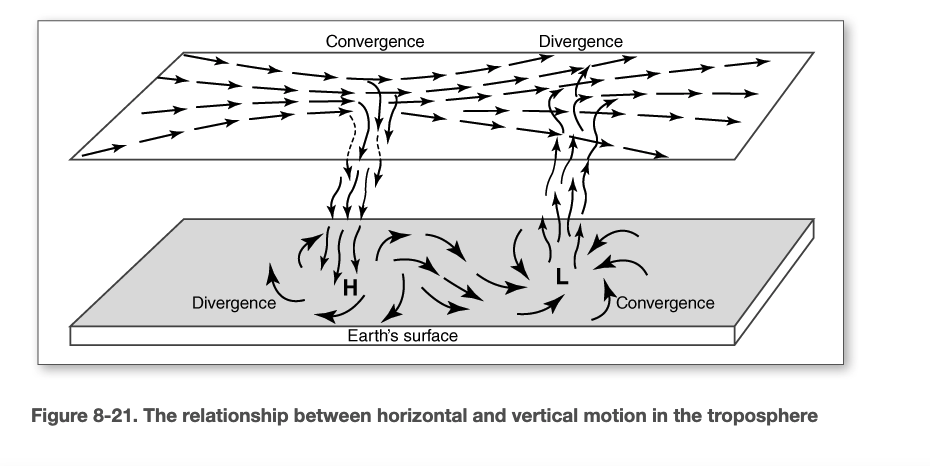
\includegraphics[width=0.5\linewidth]{uploads/relationship between lower and vertical motion.png}
\end{figure}
\begin{figure}
    \centering
    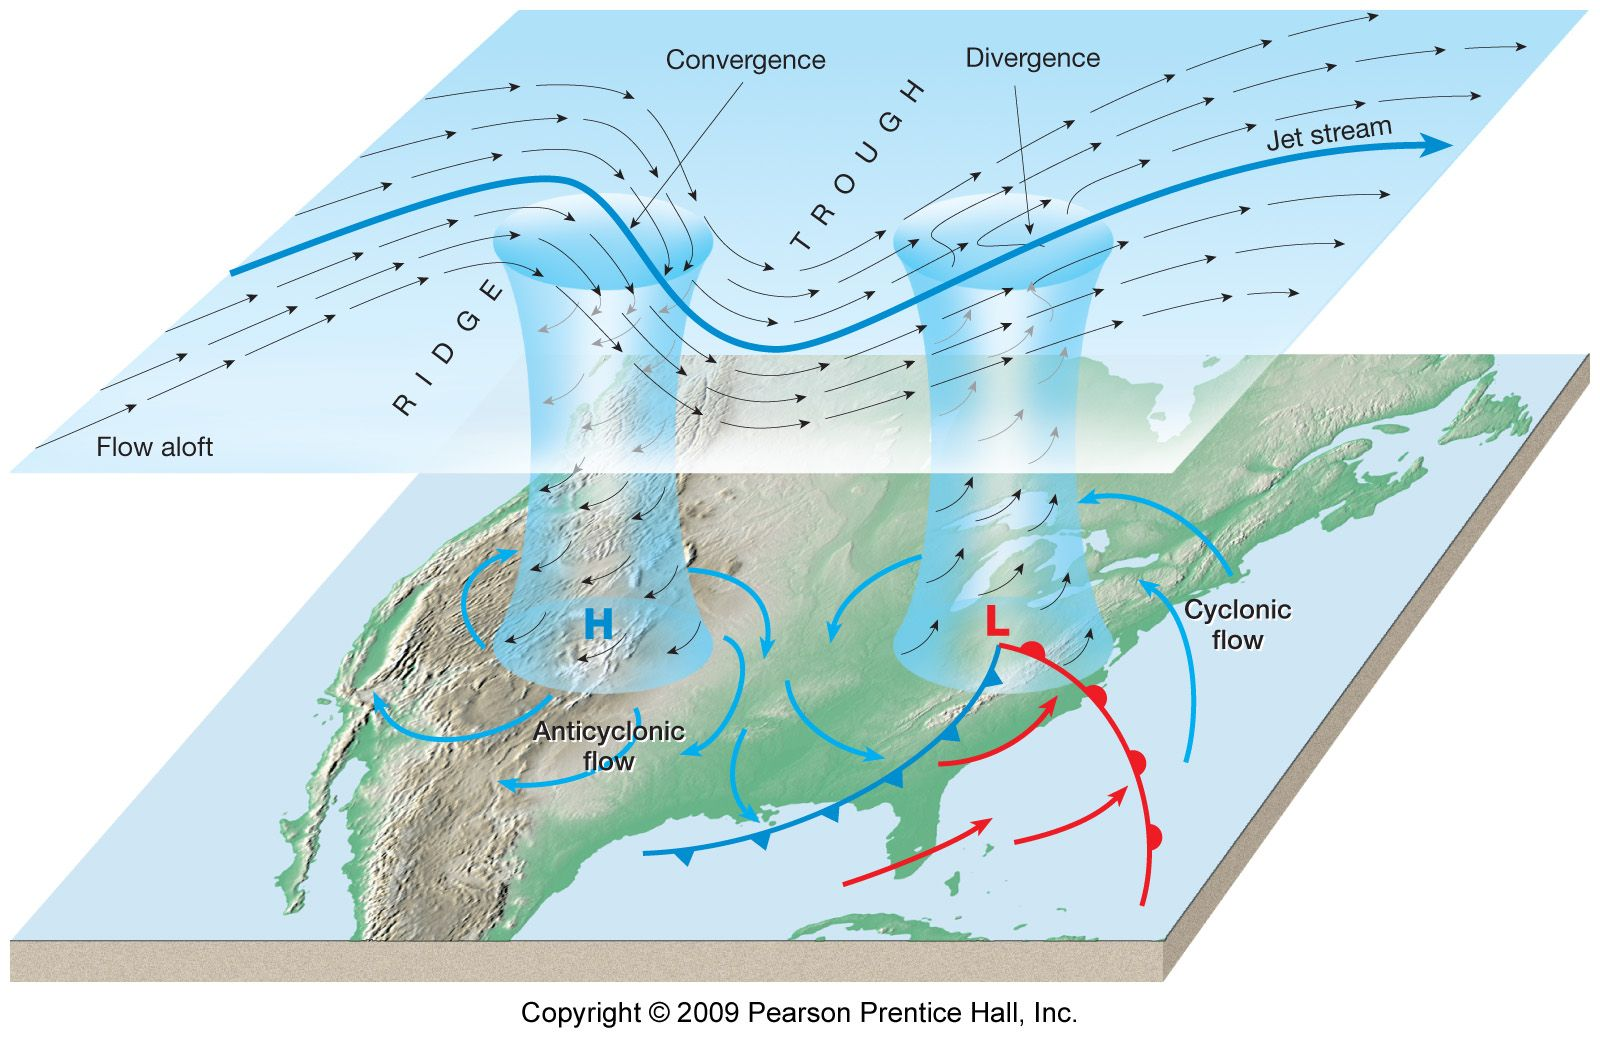
\includegraphics[width=0.5\linewidth]{through and divergence.png}
\end{figure}
\begin{figure}
    \centering
    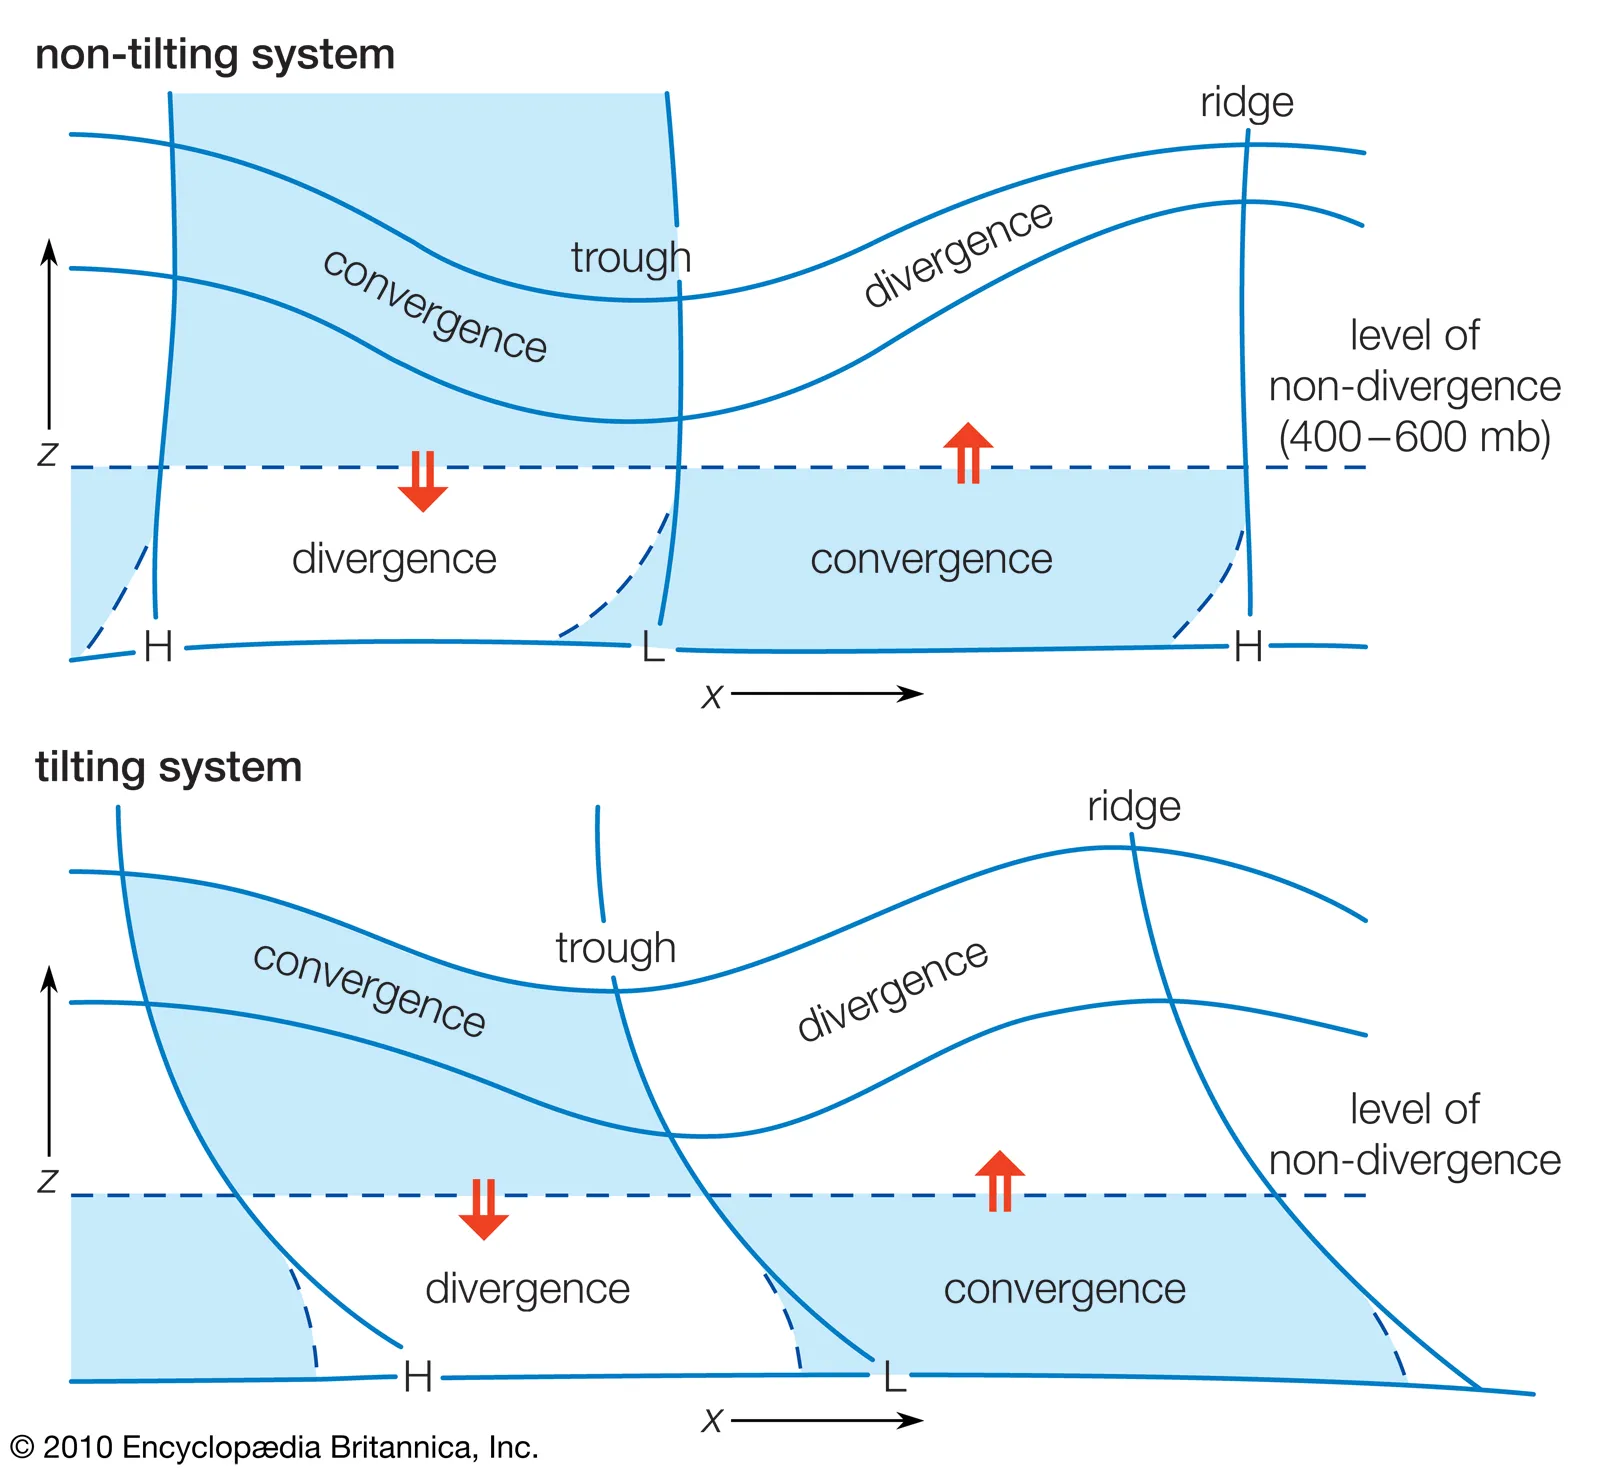
\includegraphics[width=0.5\linewidth]{uploads/conv and div.png}
\end{figure}

\section{Space-time splitting}
The dominant shape of the global circulation suggests that some understanding can be gained from splitting the physical fields into larger and smaller portions using appropriate averages. At a first inspection, the flow is seen as a predominant circumpolar vortex with superposed fluctuations in space and time. The longitudinal direction is also known as the “zonal” direction, therefore the average over longitude is known as the zonal averaging 

\subsection{Zonal mean}
The zonal mean of a quantity A is defined as the average over longitudes. Commonly used symbols in the literature are the overbar $\overline{u}$ or square brackets [u], the first is most frequently encountered in the theoretical and modeling literature whereas the second is most commonly used in observational and diagnostics works. In the following, we will use brackets. 
\begin{equation}
    [A] = \frac{1}{2\pi}\int_0^{2\pi} A \, dx
\end{equation}
so that the entire field can be decomposed in
  \begin{equation}
    A = [A] + A^*
\end{equation}
where $A^*$ is the deviation from the zonal mean. 
 The average has the properties that \([[A]] = [A]\) and \([A^*]=0\).

When a stream function can be defined, the average zonal mean meridional
velocity is zero:
\begin{equation}
    = \frac{1}{2\pi}\int_0^{2\pi} v \, dx=\frac{1}{2\pi}\int_0^{2\pi} \frac{\partial \psi}{\partial x} \, dx=0
\end{equation}


This is a consequence of the more general result that the zonal mean of
any quantity that is a longitude derivative is zero.

\subsection{Time mean}
The time mean is defined simply as the average over a length of time.
Also in this case several common symbols are used, once again the
overbar or sometimes curly brackets, in the following we will use the
overbar


\begin{equation}
    bar{A} = \frac{1}{T}\int_0^{T} A \, dt
\end{equation}

so that the total field is

\begin{equation}
    A = \bar{A} + A'
\end{equation}

The deviations from the zonal means are called "eddy" components. An
eddy that obeys a dispersion relation is a "wave".

\subsection{Higher order quantities}

The averages can be used to decompose higher-order quantities. For
instance using zonal means a quadratic correlation of the form \(A B\)
can be decomposed as

\begin{equation}
    A B = ([A]+A^*)([B]+B^*) = A^*B^* + [A] B^*+ A^*[B] + [A][B]
\end{equation}

taking a further zonal mean we get
\begin{equation}\label{eq. 2}
= [A^*B^*+ [A]B^* + A^*[B] + [A][B]] =  [A][B] + [A^*B^*]
\end{equation}

because the mix terms disappear as the average of the deviations is
zero.

We can refine the splitting by considering the time average splitting of
the zonal terms:

\begin{equation}
    = \bar{[A]} + [A]' \\
A^* = \bar{A}^* + A'^*
\end{equation}

These terms represent the stationary symmetric circulation, the
transient symmetric circulation and the stationary deviation from the
zonal means ("asymmetries") and the transient asymmetries.

Inserting these relations into Eq. \ref{eq. 2} we get


\begin{equation}
    = (\bar{[A]} + [A]')(\bar{[B]} + [B]') + [A^*B^*]
\end{equation}
    
the time mean of the terms linear in the time deviation will average
again to zero (this time with respect the time mean) and we finally get

\begin{equation}
    \overline{[AB]}) = \bar{[A]}\bar{[B]} + \overline{[A]'[B]'} + \overline{[A^*B^*]}
\end{equation}

The decompositions are not unique. We have first performed the split in
the zonal mean and then the split in the time mean, considering a split
only in the eddy part:
\begin{equation}
    A^* =    \bar{A}^* + A'^*
\end{equation}


we would get

\begin{equation}
    \overline{AB}] = \bar{[A]}\bar{[B]} +  [\bar{A}^*\bar{B}^*]+[\overline{A'^*B'^*}]
\end{equation}


where the first term is the contribution of the mean meridional
circulation, the second is the contribution of the time-mean
(standing) eddies and the last one is the contribution of the
transient eddies. This kind of decomposition is therefore a useful instrument but
requires always consideration of the hypothesis formulated in the
initial design. Another consideration is that they depend on the
specific kind of averaging that is used. There is little choice in the
zonal mean, being fixed by the geometry, but we have much more choices
in the case of the time mean. Results will depend on the length of the
time averaging period and on the original frequency of the data. Time
mean and second-order quantities calculated over daily will differ from
the same quantities calculated over time series of weekly or monthly
data. There is no \emph{correct} choice, each one will offer a different
glimpse in the data from a chosen perspective.





